\chapter{Implementation}
\section{Used Technologies}
\subsection{IntelliJ IDEA} 
The Implementation of the project is written in Java on the integrated development environment IntelliJ. It is an integrated development environment for developing Java based software. Nevertheless, it supports other programming languages too like Scala, Groovy and Kotlin. The IDE is also often used for mobile development in Android or Cordova. It could be very practicable for web development because of the following different frameworks: JavaScript, AngularJs, Node.js, TypeScript etc…
This IDE support a huge variety of benefits like:
\begin{itemize}
\item Different build systems (maven, gradle, ant, grunt, bower etc \ldots)
\item Version control systems (Git, Mercurial, Perforce, and SVN)
\item Plugin ecosystem
\item Test runner and coverage
\end{itemize}
\subsection{Maven} \label{ssec:maven}
This is a software management and build automation tool which is based on the concept of a project object modem (POM). One of the biggest feature in Maven is the dependency management. Maven automatically downloads in POM file declared libraries and plug-ins from a repository and stores them local. The local repository is a folder structure that is used as a centralized storage place for locally built artifacts and as a cache for downloaded dependencies. The Maven command mvn install builds a project and places its binaries in the local repository. Then other projects can utilize this project by specifying its coordinates in their POMs.
\subsection{SceneBuilder} \label{ssec:SceneBuilder}
JavaFX Scene Builder is a visual layout tool that generates FXML, an XML-based markup language that lets developers to quickly design user interfaces, without any coding. Users just have to drag and drop UI components to the work area. By selecting components users can easily modify their properties or apply style sheets. The code for the layout is generated automatically in the background by the tool. The resulting FXML file can be combined with a Java project by binding the UI to the application’s logic. Every item of the layout view can be assigned with an fx:id to give the controller an easy access of components by the "@FXML" annotation.  SceneBuilder is an external tool so it has to be downloaded from the official Oracle website and has to be integrated to a Java supportive IDE. 
\subsection{JavaFX}
JavaFX enables developers to design rich client applications that is able to run constantly on different platforms. It offers a wide range of APIs for web rendering, user interface styling and media streaming. The newest JavaFX releases are fully integrated with the Java SE 7 Runtime Environment, which is available for all main desktop platforms. and the Java development Kit. So JavaFX application compiled to JDK 7 or later also run on all major desktop. 
\section{Surrounding packages}
The NoBeardMachine is part of the existing NoBeard project. This project already consists of the following packages:
\begin{itemize}
\item \textbf{asm: }NoBeard Assembler to assemble .na files 
\item \textbf{compiler: }NoBeard Compiler to compile .nb source code files
\item \textbf{config: }Returns the version of the NoBeard project
\item \textbf{error: }To handle errors that are acquiring during compilation or assembly   
\item \textbf{io: }Responsible for reading source files and handling binary files 
\item \textbf{machine: }Implements a virtual machine with components like DataMemory, ProgramMemory, Instructions etc...  
\item \textbf{parser: }Converts source code files to binary files
\item \textbf{scanner: }To analyze NoBeard source code files for keywords, operands or arguments  
\item \textbf{symbolTable: }Looks up for matching words based on the symbol table entry  
\end{itemize}
However, one of the most important package is the “machine”. This is defined as the core of the whole project because it has the most significantly roles such as running a NoBeard program.
\section{Architecture of the User Interface}
The GUI is designed very similar to the Model-View-Controller pattern. However, this project is not depending on any database so it comes without any Model. The GUI project is build up of three main components as shown in figure~\ref{fig:partsOfGui}. The Controller and the Virtual Machine both of them is running on different threads and are accordingly synchronized. This will be described in detail in section~\ref{synchronization}. The relationship between the controller and view is for event actions and updating of view-components like data memory, output or program flow. The View allows users to call functions from the Controller by clicking on control buttons or by entering inputs. 
\begin{figure}[h] 
	\centering
	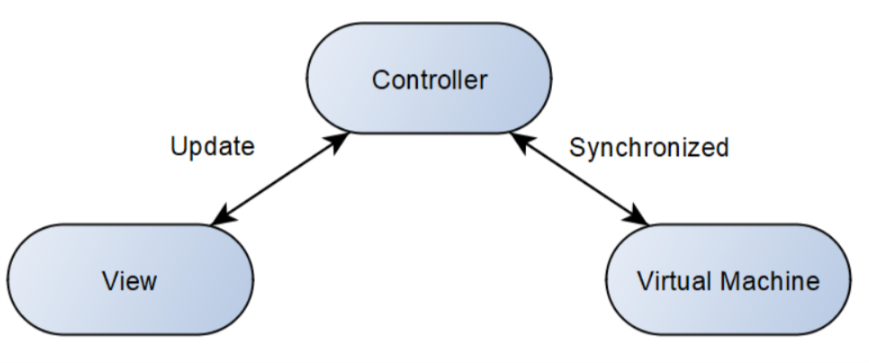
\includegraphics[scale=.70]{images/modelOfGui.png}
	\caption{Main parts of the GUI implementation}
	\label{fig:partsOfGui}
\end{figure}
\subsection{The View}
The view is a single fxml file which holds the view components of the layout. It was created with an external tool called SceneBuilder which is already described in section~\ref{ssec:SceneBuilder}. Each window is made up of an AnchorPane and is separated by SplitPanes. AnchorPane enables developers to construct high rated dynamic user interfaces for desktops. It is a highly specialized layout that can be used for edge alignment. This benefit gives the possibility to fill the whole pane to the parent, which is a SplitPane, by setting anchor offsets to zero. So, it becomes very comfortable and easy to size every window as the user wants. Then each of these AnchorPanes holds the needed view-components like Button, TextArea, TextField, ListView or ScrollPane. 
\subsection{The Controller}
The controller is primarily responsible for the coordination and operation of the view and its components. As already described in section~\ref{ssec:SceneBuilder} the controller can have easy access to the view components via the binding of an fx id. But firstly, they have to be connected with each other by setting the "fx:controller" attribute of the root view element to the currently used controller. Through this advantage it does not need to now the resource file of the layout or to call any "get" functions to get the target items. Even event actions, like mouse click or key pressing, can be bound between the controller and the view. This could be achieved by setting a name for the "On Action" property in SceneBuilder and then creating the related function in the controller. The function has to be declared with the "@FXML" annotation and the same name as it was set on the action property of the item. Even functions like this comes only with a single argument which an ActionEvent. This parameter could be very helpful for getting some further information of the fired event like which mouse button was pressed.

\section{Synchronization of NoBeard Machine and GUI}
\label{synchronization} 
Initially, it gets an instance of the NoBeard machine where simple program can be executed. The opening of a NoBeard object file is operated with the help of a BinaryFileHandler. After a successful opening of the object file, it has to be disassemble. This function converts binary files to primary program data where addresses, instructions and operands become visible on the UI.
By finishing the translation, the machine has to load the string storage and the program from the object file. Program data is filled in a VBox with a CheckBox and text of the data for every line. All of the CheckBoxes gets an OnAction event which add and remove breakpoints from the machine. 
On starting a program, a new external thread has to be started where the machine runs separate from the UI. Its executes step by step every instruction of the program until any interruptions. It can be interrupted by a breakpoint, input request or by a halt instruction.
\section{Handling of Breakpoints (Break instruction)}
Machine internal handling of breakpoints is done as described in \cite{bendersky_how_nodate}.

The implementation for the maintaining of breakpoints is coded with a simple observer pattern design to achieve the best performance of the virtual machine. The machine is completely separated from the breakpoint stuff. It runs only until its state equals to “running”. So, a new instruction is introduced, called “BREAK”, which sets the machine in to a “blocked” state. The ControlUnit which is responsible for execution cycles in the virtual machine is going to be an Observable. Then a new Observer class is implemented which is called debugger that is holding all breakpoints in a HashMap. This HashMap stores the address and the instruction of a breakpoint. The debugger class contains in all three major functions. Adding, removing breakpoints to the HashMap and replacing an instruction at a specified address from the program memory to a new one. The selection of a breakpoint on the UI calls the set or remove function from the debugger, as the case may be. As soon as a breakpoint is selected, it will be stored to the HashMap with its original instruction and at same time replaces the original instruction by the newly added break instruction. This break instruction set the machine to a blocked state and notify the observer to change the break instruction back to the original one which is stored in the HashMap. Now the machine is blocked at a specified breakpoint and the user can take a look to the current stack frames and go one step further in the program or continue the execution cycle to a next breakpoint. However, when the user wants to step further to execute the current instruction where the breakpoint is, a switch back to the break instruction is needed again after the original instruction completed.  
\section{Interruption by input request (Threading)}
As already mentioned, the virtual machine runs on a separate thread so every time the user has to operate an input, a switch to the UI thread is needed. Otherwise it would cause a critical section between the threads. The synchronization of these two threads is implemented with the semaphore construction. The NoBeardMachine contains two interfaces to optimize outputs and inputs on the used device. As soon as the machine executes an input instruction (IN), it calls firstly a function from the input interface either hasNextInt() or hasNext(). Both do the same thing, checks whether there is an input by the user or not. The only different is that the one of them also checks if the string is numeric. These functions are overridden in the FxInputDevice class where also an instance of the controller is loaded by the constructor. So, by calling one of these hasNext function the machine thread should be paused. To avoid the deadlock, the semaphore from the controller is acquired at this position. Now the user can make an input on the FX thread and submit it. To get back to the machine thread, the semaphore hast to be released after the user fires the submit event by pressing the ENTER key. Then the machine continues at the same position where the semaphore was acquired, at one of the has Next function and can analyse the provided input string.
\section{Visualisation of DataMemory}
\label{sec:implementationOfDataVisualisation}
To visualize data like string constants or local variables of the current frame from the data memory a listView is defined on the view. Firstly a function iterates through the dataMemory until the current stack pointer and groups all data into four bytes and finally stores them into an observable collection of strings. Of course, after each break this list view has to be updated to the current stack. Each row of the list view contains a line of string, for example by calling the getItem() function it should return a collection of strings for every row. So the translation for one byte is impossible because one row contains for byte data. Now one row of the list view will be separated in four labels with one byte. These labels get a click event to open up a context menu where four functions are available. For the implementation of these functions a separated DataMemoryConverter class is introduced. The conversion of a single byte to character is handled by translating the ASCII value which is the current byte to a char.


As already mentioned in section~\ref{ssec:dataMemory} integers are stored in little endian order, that means the lowest significant byte is stored first. 